
% part 16
\section{Демонизация Twisted\label{sec:part16}}

\subsection{Введение}


Серверы, которые мы написали до сих пор, запускались только 
в терминальном окне, с выводом на экран через оператор 
print. Это подходит для программы на стадии разработки, но 
это едва ли подходит для релизов. Хорошо написанная программа, 
готовая для выкладке, должа:

\begin{enumerate}

\item Запускаться как 
\href{http://en.wikipedia.org/wiki/Daemon\_%28computer_software%29}{демон}, отсоединяясь от 
любой терминальной или пользовательской сессии. Сервис 
не должен завершаться после того, как 
администратор отлогился.

\item Отправлять отладочный и ошибочный вывод во 
множество ротируемых лог файлов или в сервис 
\href{http://en.wikipedia.org/wiki/Syslog}{syslog}.

\item Убирать лишние привилегии, например, переключаться к 
к низкопривелигированному пользователю до запуска.

\item Записывать свой 
\href{http://en.wikipedia.org/wiki/Process\_ID}{pid} в файл так, чтобы администратор 
мог без проблем 
\href{http://en.wikipedia.org/wiki/Kill%28%29}{отправить сигналы} в демон.

\end{enumerate}


Мы можем добраться до всех этих вещей, 
используя скрипт twistd, предоставляемый Twisted. Но сначала, 
мы должны быть немного поменять наш код.


\subsection{Концепции}

%Understanding twistd will require learning a few new concepts in Twisted, the most important being a Service. As usual, several of the new concepts are accompanied by new Interfaces.
Для того, чтобы понять twisted, необходимо изучить несколько 
новых понятий в Twisted, наиболее важное из них - Service. Как всегда, 
несколько новых концепций сопровождаются новыми Interface'ми.

\subsubsection{IService}

%The IService interface defines a named service that can be started and stopped. What does the service do? Whatever you like — rather than define the specific function of the service, the interface requires only that it provide a small set of generic attributes and methods.

Интерфейс 
\href{http://twistedmatrix.com/trac/browser/tags/releases/twisted-10.0.0/twisted/application/service.py#L87}{IService} опредлеяет именнованный сервис, 
который может быть запущен и остановлен. 
Интерфейс требует наличия небольшого 
множества основных атрибутов и методов.


Существует два обязательных атрибута: name и running. 
Атрибут name - это просто строка, например 'fastpoetry', или 
None, если вы не хотите давать Вашему сервису название. 
Атрибут running - булево значение, которое устанавливается в true, 
если сервис успешно запущен.


Мы собираемся коснуться лишь некоторых методов IService. 
Мы пропустим некоторые, являющиеся очевидными, и другие, которые 
наиболее продвинуты и в основном не используются в простых 
Twisted программах. Два основных метода IService - 
\href{http://twistedmatrix.com/trac/browser/tags/releases/twisted-10.0.0/twisted/application/service.py#L130}{startService} и 
\href{http://twistedmatrix.com/trac/browser/tags/releases/twisted-10.0.0/twisted/application/service.py#L135}{stopService}:

\begin{scriptsize}\begin{verbatim}
    def startService():
        """
        Start the service.
        """

    def stopService():
        """
        Stop the service.

        @rtype: L{Deferred}
        @return: a L{Deferred} which is triggered when the service has
            finished shutting down. If shutting down is immediate, a
            value can be returned (usually, C{None}).
        """

\end{verbatim}\end{scriptsize}

Что эти методы делают будет зависеть от сервиса. Например, 
метод startService может любое из:

\begin{itemize}
\item Загружать некоторые конфигурационные данные
\item Инициализировать базу данных
\item Начать слушать порт
\item Ничего не делать 
\end{itemize}


Метод stopService может:

\begin{itemize}
\item Сохранять некоторое состояние
\item Закрывать открытие соединения к базе данных
\item Завершать слушать порт
\item Ничего не делать 
\end{itemize}


Когда мы пишем наши пользовательские сервисы, мы должны 
соответсвующе реализовать эти методы. 
Для некоторых общих случаев, подобно прослушиванию порта, 
Twisted предоставляет готовые сервисы, которые мы можем использовать. 


Заметим, что stopService может опционально возвратить deferred, 
который нужно активизировать, когда сервис окончательно 
прекратил работать. Это позволяет нашим сервисам убрать за собой 
до того как приложение завершится. Если Ваш сервис сразу же завершается, 
вы можете возвратить None вместо deferred'а.  


Сервисы могут быть организованы в коллекции, которые вместе  
стартуют и завершаются. Последний метод IService, на который мы будем 
смотреть - 
\href{http://twistedmatrix.com/trac/browser/tags/releases/twisted-10.0.0/twisted/application/service.py#L107}{setServiceParent}, добавляет Service в коллекцию:

\begin{scriptsize}\begin{verbatim}
    def setServiceParent(parent):
        """
        Set the parent of the service.

        @type parent: L{IServiceCollection}
        @raise RuntimeError: Raised if the service already has a parent
            or if the service has a name and the parent already has a child
            by that name.
        """
\end{verbatim}\end{scriptsize}


Любой сервис может иметь родительский, что означает, что 
сервисы могут быть организованы в иерархию. И это подводит нас 
к следующему Interface'у, на который мы собираемся сегодня посмотреть.


\subsubsection{IServiceCollection}

The IServiceCollection interface defines an object which can contain IService objects. A service collection is a just plain container class with methods to:


Интерфейс \href{http://twistedmatrix.com/trac/browser/tags/releases/twisted-10.0.0/twisted/application/service.py#L203}{IServiceCollection} определяет объект, который 
может содержать объекты IService. Коллекция сервисов - просто 
обычный контейнерный класс с методами:

\begin{itemize}

\item Искать сервис по названию (\href{http://twistedmatrix.com/trac/browser/tags/releases/twisted-10.0.0/twisted/application/service.py#L212}{getServiceNamed})

\item Пройтись по всем сервисам в коллекции (\href{http://twistedmatrix.com/trac/browser/tags/releases/twisted-10.0.0/twisted/application/service.py#L222}{\_\_iter\_\_})

\item Добавить сервис в коллекцию (\href{http://twistedmatrix.com/trac/browser/tags/releases/twisted-10.0.0/twisted/application/service.py#L227}{addService})

\item Удалить сервис из коллекции (\href{http://twistedmatrix.com/trac/browser/tags/releases/twisted-10.0.0/twisted/application/service.py#L236}{removeService})

\end{itemize}


Заметим, что реализация IServiceCollection не 
является автоматически реализацией IService, 
но нет препятсвий одному классу реализовать 
оба интерфейса (и мы увидим пример).


\subsubsection{Application}

Twisted Application не определяется отдельным интерфейсом. 
Скорее, объект Application требуется для реализации обоих 
IService и IServiceCollection, также как и для нескольких других, 
которые мы собираемся рассмотреть. 


Приложение - это сервис верхнего уровня, который представляет 
наше полное Twisted приложение. Все другие сервисы в вашем 
демоне будут детьми (или внуками, и т.д.) объекта Application. 


Редко, когда надо реализовывать свое собственное Application. 
Twisted предоставляет реализацию, которую мы будем 
сегодня использовать.

\subsubsection{Twisted логирование}


Twisted включает свое собственную инфраструктуру логирования в модуле 
\href{http://twistedmatrix.com/trac/browser/tags/releases/twisted-10.0.0/twisted/python/log.py}{twisted.python.log}. Основные API для записи в лог простые, поэтому мы просто 
включим небольшой пример, расположенный в 
basic-twisted/log.py, и вы можете просмотреть интересующие Вас детали 
в соответсвующем модуле Twisted.


Мы не будем вам докучать, показывая API для установки логирующих 
обработчиков, поскольку twistd делает это за нас.

\subsection{FastPoetry 2.0}

Хорошо, давайте взглянем на некоторый код. Мы обновили 
наш поэтический сервер для того, чтобы запускать его с 
помощью twistd. Его исходный код расположен в 
\href{http://github.com/jdavisp3/twisted-intro/blob/master/twisted-server-3/fastpoetry.py#L1}{twisted-server-3/fastpoetry.py}. Сначала мы посмотрим на 
\href{http://github.com/jdavisp3/twisted-intro/blob/master/twisted-server-3/fastpoetry.py#L9}{PoetryProtocol}:

\begin{scriptsize}\begin{verbatim}
class PoetryProtocol(Protocol):

    def connectionMade(self):
        poem = self.factory.service.poem
        log.msg('sending %d bytes of poetry to %s'
                % (len(poem), self.transport.getPeer()))
        self.transport.write(poem)
        self.transport.loseConnection()

\end{verbatim}\end{scriptsize}

%Notice instead of using a print statement, we’re using the twisted.python.log.msg function to record each new connection.
Заметьте, что вместо использования оператора print, 
мы используем функцию twisted.python.log.msg для 
записи каждого соединения.
Далее класс \href{http://github.com/jdavisp3/twisted-intro/blob/master/twisted-server-3/fastpoetry.py#L19}{PoetryFactory}:

\begin{scriptsize}\begin{verbatim}
class PoetryFactory(ServerFactory):

    protocol = PoetryProtocol

    def __init__(self, service):
        self.service = service
\end{verbatim}\end{scriptsize}

%As you can see, the poem is no longer stored on the factory, but on a service object referenced by the factory. Notice how the protocol gets the poem from the service via the factory. Finally, here’s the service class itself:

Как вы видите, поэма больше не хранится в PoetryFactory, 
вместо этого она хранится в сервисном объекте, на которую 
есть ссылка из PoetryFactory. Заметьте, как PoetryProtocol получает 
поэму из service через factory. Наконец, далее сам 
\href{http://github.com/jdavisp3/twisted-intro/blob/master/twisted-server-3/fastpoetry.py#L27}{сервисный класс}:

\begin{scriptsize}\begin{verbatim}
class PoetryService(service.Service):

    def __init__(self, poetry_file):
        self.poetry_file = poetry_file

    def startService(self):
        service.Service.startService(self)
        self.poem = open(self.poetry_file).read()
        log.msg('loaded a poem from: %s' % (self.poetry_file,))
\end{verbatim}\end{scriptsize}


Так же как и с другими многочисленными классами Interface, 
Twisted предоставляет базовый класс, который мы можем 
использовать для того, чтобы сделать нашу 
собственную реализацию используя поведение по 
умолчанию. Здесь мы используем класс 
\href{http://twistedmatrix.com/trac/browser/tags/releases/twisted-10.0.0/twisted/application/service.py#L154}{twisted.application.service.Service} для реализации 
нашего PoetryService.


Базовый класс предоставляет реализацию по умолчанию 
всех необходимых методов, поэтому нам нужно 
реализовать только пользовательское поведение. В нашем случае, 
мы просто перегружаем startService для 
загрузки файла с поэзией. Заметим, что мы все равно вызываем 
метод базового класса (который устанавливает для нас 
атрибут running).


Другая сторона здесь плохо упомянута. Объект PoetryService 
не знает ничего о деталях PoetryProtocol. Сервис только 
должен загрузить поэму и обеспечить доступ до него любого 
объекта, который нуждается в поэме. Другими словами, 
PoetryService обеспокоен только высокоуровневыми деталями 
в преоставлении поэзии, а не низкоуровневыми деталями 
отправки по TCP соединению. Таким образом, этот сервисный 
класс мог бы быть использован другим протоколом, скажем UDP или 
XML-RPC. В случае нашего простого сервиса пользы от этого мало, 
но можно представить преимущества в более реалистичной сервисной реализации. 


Если бы это была обычная Twisted программа, весь код, 
на который мы посмотрели до сих пор не был бы в одном файле, 
он был бы в нескольких разных модулях (возможно, 
fastpoetry.protocol и fastpoetry.service). Но, следуя нашей 
обычной практике создания примеров самодостаточными, мы 
включаем все что нам надо в один скрипт.

\subsubsection{Twisted tac файлы}

Оставшийся код в скрипте содержит то, 
что обычно бывает содержимым Twisted tac файла. 
Файл tac - Twisted Application Configuration файл, который 
говорит twistd как создавать приложение. Поскольку это 
конфигурационный файл, то он ответственнен за выбор настроек (подобно 
номерам портов, расположениями файлов с поэзией и т.д.) для 
запуска приложения определенным образом. Другими словами, 
tac файл представляет определенный вид запуска для нашего сервиса (обслужить 
эту поэму на этом порту), а не общий скрипт для 
запуска любого поэтического сервера.


Если бы мы запускали несколько поэтических сервером на одной 
машине, мы бы имели несколько tac файлов для каждого (вот почему 
tac файлы обычно не содержат кода общего назначения). В нашем примере, 
tac файл сконфигурирован для обслуживания poetry/ecstasy.txt на 
порту 10000 loopback интерфейса:

\begin{scriptsize}\begin{verbatim}
# configuration parameters
port = 10000
iface = 'localhost'
poetry_file = 'poetry/ecstasy.txt'
\end{verbatim}\end{scriptsize}


Заметим, что twistd ничего не знает об этих переменных, 
мы их определяем здесь для того, чтобы сохранить все наши 
конфигурационные переменные в одном месте. Фактически, twistd заботится 
только об одной переменной во всем файле, как мы это вскоре поймем. 
Далее мы \href{http://github.com/jdavisp3/twisted-intro/blob/master/twisted-server-3/fastpoetry.py#L44}{начинаем} построение нашего приложения:

\begin{scriptsize}\begin{verbatim}
# this will hold the services that combine to form the poetry server
top_service = service.MultiService()
\end{verbatim}\end{scriptsize}


Наш поэтический сервер состоит из двух 
сервисов: PoetryService, который мы определили выше, и 
встроенный Twisted сервис, который создает слушающий сокет 
нашей поэмы, из которого она будет предоставляться. Поскольку 
эти два сервисы очевидным образом связаны друг с другом, 
мы сгруппируем их вмести, используя \href{http://twistedmatrix.com/trac/browser/tags/releases/twisted-10.0.0/twisted/application/service.py#L253}{MultiService} - класс Twisted, 
который реализует IService вместе с IServiceCollection.


Будучи сервисной коллекцией, MultiService сгруппирует 
наши два поэтических сервиса вместе. И будучи сервисом, 
MultiService запустит оба дочерних сервиса, когда 
MultiService сам запустится, и остановит их, когда сам остановится. 
Давайте добавим наш первый поэтический сервис в коллекцию:

\begin{scriptsize}\begin{verbatim}
# the poetry service holds the poem. it will load the poem when it is
# started
poetry_service = PoetryService(poetry_file)
poetry_service.setServiceParent(top_service)
\end{verbatim}\end{scriptsize}


Эта достаточно удобная вещь. Мы только создаем 
PoetryService и затем добавляем его в коллекцию, 
используя setServiceParent, который унаследован из 
базового класса Twisted. Затем мы \href{http://github.com/jdavisp3/twisted-intro/blob/master/twisted-server-3/fastpoetry.py#L53}{слушаем} TCP сокет:

\begin{scriptsize}\begin{verbatim}
# the tcp service connects the factory to a listening socket. it will
# create the listening socket when it is started
factory = PoetryFactory(poetry_service)
tcp_service = internet.TCPServer(port, factory, interface=iface)
tcp_service.setServiceParent(top_service)
\end{verbatim}\end{scriptsize}


Twisted предоставляет сервис TCPServer для создания 
слушающего TCP сокета, присоединенного к 
произвольной factory (в нашем случае - PoetryFactory). 
Мы не вызываем reactor.listenTCP напрямую, поскольку 
работа tac файла - сделать наше приложение готовым к старту 
не запуская его. TCPServer создаст сокет после того, как 
он запустится скриптом twistd.  


Вы могли заметить, что мы не беспокоились заданием 
названия сервиса. Именование сервисов не является 
обязательным, а наоборот - опциональным свойством, 
которое вы можете использовать, если хотите 
<<просматривать>> сервисы во время запуска. Поскольку 
нам не нужно этого делать в нашем маленьком приложении, 
то мы не беспокоимся об этом.


Хорошо, мы получили оба наших сервиса, объединенных 
в коллекцию. Теперь мы только сделаем Application и 
добавим нашу коллекцию в него:

\begin{scriptsize}\begin{verbatim}
# this variable has to be named 'application'
application = service.Application("fastpoetry")

# this hooks the collection we made to the application
top_service.setServiceParent(application)
\end{verbatim}\end{scriptsize}


Единственная переменная в этом скрипте, которая 
интересует twistd - переменная application. Это то, как 
twistd найдет приложение, которое предполагается запустить (поэтому 
переменная должна иметь название "application"). И когда 
приложение запустится, все сервисы, которые мы туда добавили, 
также будут запущены.


На рисунке \ref{fig:application} показана структура приложения, 
которое мы только что построили:

\begin{figure}[h]
\begin{center}
    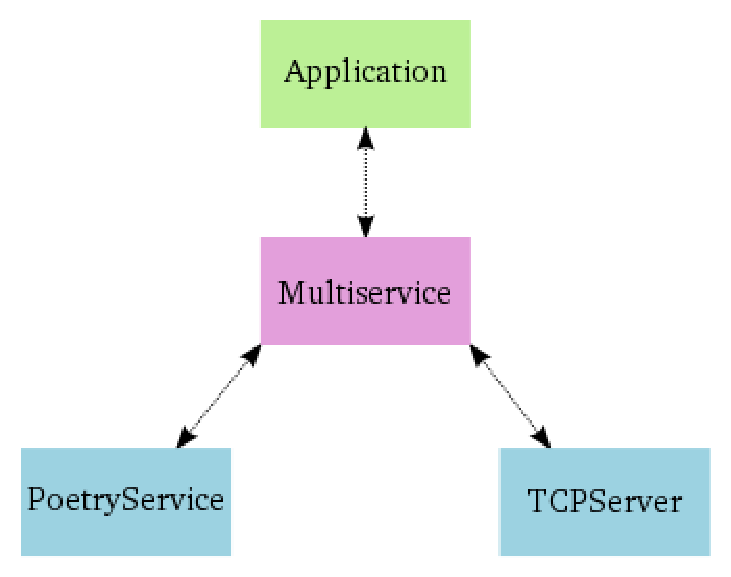
\includegraphics[width=0.5\textwidth]{images/application.pdf}
    \caption{Структура fastpoetry приложения\label{fig:application}}
\end{center}
\end{figure}


\subsubsection{Запуск сервера}


Давайте запустим наш сервер. 
Поскольку наш скрипт - tac файл, то нам нужно запустить его с помощью twistd.  
Конечно же, tac файлы - обычные Python скрипты. 
Давайте сначала запустим tac файл без twistd, 
просто используя интерпретатор Python и посмотрим, что получается:

\begin{scriptsize}\begin{verbatim}
python twisted-server-3/fastpoetry.py
\end{verbatim}\end{scriptsize}


Если вы сделаете это, вы обнаружите, что ничего не произошло! 
Как мы говорили до этого, работа tac файла - сделать приложение 
готовым для запуска, без его запуска. В качестве напоминание об этом 
специальном назначении tac файлов, некоторые люди называют их с 
расширением .tac вместо .py. Скрипт twistd не заботится о 
расширении файла.


Давайте запустим наш сервер по-настоящему, используя twistd:

\begin{scriptsize}\begin{verbatim}
twistd --nodaemon --python twisted-server-3/fastpoetry.py
\end{verbatim}\end{scriptsize}


После запуска такой команды вы увидите похожий вывод:

\begin{scriptsize}\begin{verbatim}
2010-06-23 20:57:14-0700 [-] Log opened.
2010-06-23 20:57:14-0700 [-] twistd 10.0.0 (/usr/bin/python 2.6.5) starting up.
2010-06-23 20:57:14-0700 [-] reactor class: twisted.internet.selectreactor.SelectReactor.
2010-06-23 20:57:14-0700 [-] __builtin__.PoetryFactory starting on 10000
2010-06-23 20:57:14-0700 [-] Starting factory <__builtin__.PoetryFactory instance at 0x14ae8c0>
2010-06-23 20:57:14-0700 [-] loaded a poem from: poetry/ecstasy.txt
\end{verbatim}\end{scriptsize}

Здесь нужно отметить несколько вещей:

\begin{enumerate}

\item вы видите вывод системы логирования Twisted, в том числе вызов 
log.msg в PoetryFactory. Но мы не устанавливали logger в нашем tac 
файле, так как twistd должен это сделать для нас.  

\item вы также можете увидеть, что наши два основных сервиса, PoetryService и TCPServer,
запустились.

\item Командная строка не возвращается. Это означает, что наш сервер 
не запущен как демон. По умолчанию, twistd запускает сервер как демон (это 
основная причина существования twistd), но если вы используете опцию 
--nodaemon, то twistd запустит ваш сервер как обычный консольный процесс, и 
лог будет выводится на стандартный вывод. Это полезно при отладки ваших 
tac файлов.

\end{enumerate}


Теперь протестируем сервер путем скачивания поэмы одним из 
наших поэтических клиентов или даже netcat'м:

\begin{scriptsize}\begin{verbatim}
netcat localhost 10000
\end{verbatim}\end{scriptsize}

Такая команда должна скачать поэму из сервера, и вы 
увидите новую запись в логе подобную такой: 

\begin{scriptsize}\begin{verbatim}
2010-06-27 22:17:39-0700 [__builtin__.PoetryFactory] sending 3003 bytes of poetry to IPv4Address(TCP, '127.0.0.1', 58208)
\end{verbatim}\end{scriptsize}


Эта запись появляется в результате вызова log.msg в 
PoetryProtocol.connectionMade. Если вы сделаете еще запросы к 
серверу, то на каждый запрос вы увидите новую запись в логе.


Теперь остановим сервер, нажав Ctrl-C. вы должны увидеть строки подобные:

\begin{scriptsize}\begin{verbatim}
^C2010-06-29 21:32:59-0700 [-] Received SIGINT, shutting down.
2010-06-29 21:32:59-0700 [-] (Port 10000 Closed)
2010-06-29 21:32:59-0700 [-] Stopping factory <__builtin__.PoetryFactory instance at 0x28d38c0>
2010-06-29 21:32:59-0700 [-] Main loop terminated.
2010-06-29 21:32:59-0700 [-] Server Shut Down.
\end{verbatim}\end{scriptsize}


Как вы видите, Twisted не просто разрушается, а завершает сам 
себя чисто и говорит вам о завершении в логе. Заметим, что два 
наших основных сервис также сами себя завершают.


Хорошо, теперь запустим сервер еще раз:

\begin{scriptsize}\begin{verbatim}
twistd --nodaemon --python twisted-server-3/fastpoetry.py
\end{verbatim}\end{scriptsize}


Откройте другую консоль и зайдите в директорию twisted-intro. 
В директории должен появится файл twistd.pid. Этот файл создан 
twistd и содержит идентификатор процесса нашего запущенного 
сервера. Попробуйте запустить эту команду для завершения сервера: 

\begin{scriptsize}\begin{verbatim}
kill `cat twistd.pid`
\end{verbatim}\end{scriptsize}

Заметьте, что twistd стирает файл с pid'м, когда наш сервис завершается.


\subsubsection{Реальный демон}


Теперь давайте запустим наш сервер как 
демон, который даже проще сделать, поскольку 
по умолчанию twistd демонизирует процесс:

\begin{scriptsize}\begin{verbatim}
twistd --python twisted-server-3/fastpoetry.py
\end{verbatim}\end{scriptsize}


На этот раз мы сразу же получаем командную строку обратно. 
Если вы посмотрите на содержимое вашей директории, 
то в дополнение к файлу twistd.pid, созданное для сервера, 
который мы только что запустили, вы увидите файл с 
логами --- twistd.log, который отображает тоже самое, что и 
ранее отображалось в консоли.


При запуске демона, twistd устанавливает обработчик логов, 
который пишет в файл вместо стандартного вывода. Лог-файл 
по умолчанию --- это twistd.log, расположенный в той же 
директории, где вы запустили twistd, но, если вы хотите, то 
можете менять файл использованием опции \textit{\symbol{45}\symbol{45}logfile}. 
Обработчик, который устанавливает twistd также ротирует лог, 
когда размер превышает один мегабайт.


Вы можете увидеть запущенный сервер, просмотрев список 
всех процессов в вашей системе. Продолжим и проверим 
сервер, скачав еще одну поэму. Вы увидите новые записи 
в лог файле для каждого запроса на скачивание поэмы.


Поскольку сервер больше не присоединен к консоли (и 
другим процессам, кроме init), вы не можете завершить его 
нажав Ctrl-C. Как реальный демон, процесс продолжит работу, 
даже если вы отлогинетесь. Но мы все еще можем использовать 
файл twistd.pid, чтобы остановить процесс:

\begin{scriptsize}\begin{verbatim}
kill `cat twistd.pid`
\end{verbatim}\end{scriptsize}


И когда это происходит, то в логе появляются 
сообщения об остановке сервера, файл twistd.pid 
удаляется, и наш сервер завершается.


Это хорошая идея проверить другие опции twistd. 
Например, вы можете сказать twistd переключиться на 
другого пользователя или группу до запуска демона (это 
типичный случай понижения привелегий Вашего сервера, 
которые ему не нужны, в качестве меры предосторожности). 
Мы не будем беспокоиться тщательным изучением этих 
дополнительных опций, вы можете найти их, используя 
опцию --help. 


\subsection{Системы плагинов в Twisted}

Хорошо, теперь мы можем использовать twistd для запуска 
наших серверов как подлинных демонов. Это все очень 
здорово, и тот факт, что наш ``конфигурационные'' файлы 
являются реально файлами с исходниками на Python'е, дает 
нам огромную гибкость во многих вещах. Но, нам не всегда 
нужно так много гибкости. Для наших поэтических серверов, 
обычно мы заботимся только о нескольких опциях:

\begin{enumerate}
\item Поэма для обслуживания
\item Порт для обслуживания поэмы
\item Интерфейс для прослушивания
\end{enumerate}


Создавать новые tac файлы с простыми изменениями 
переменных кажется чрезмерным. Система плагинов в 
Twisted позволяет нам сделать тоже самое.


Twisted плагины предоставляют способ 
определения именованных приложений с 
пользовательскими опциями, которые 
twistd может автоматически распознать и 
запустить. Twisted сам построен из 
множества встроенных плагинов. вы можете 
их увидеть, запуская twisted без аргументов. Попробуйте 
запустить сейчас вне директории twisted-intro. 
После раздела с помощью, вы увидите вывод подобный:

\begin{scriptsize}\begin{verbatim}
    ...
    ftp                An FTP server.
    telnet             A simple, telnet-based remote debugging service.
    socks              A SOCKSv4 proxy service.
    ...
\end{verbatim}\end{scriptsize}


Каждая строка показывает один из встроенных плагинов из Twisted. 
И вы можете любой из них, используя twistd.


Каждый плагин также имеет свое множество опций, которые вы 
можете изучить, используя опицию --help. Давайте посмотрим, 
какие опции имеет плагин ftp:

\begin{scriptsize}\begin{verbatim}
twistd ftp --help
\end{verbatim}\end{scriptsize}

Заметим, что нужно поместить опцию --help после команды 
ftp, поскольку вам нужны опции ftp, а не опции twistd.
вы можете запустить ftp сервер с помощью twistd также, 
как мы запускали наш поэтический сервер. Но, поскольку это 
плагин, то мы запускаем его по его названию:

\begin{scriptsize}\begin{verbatim}
twistd --nodaemon ftp --port 10001
\end{verbatim}\end{scriptsize}


Эта команда запускает ftp плагин в недемонизированном виде 
на порту 10001. Заметим, что опция twistd 
\textit{\symbol{45}\symbol{45}nodaemon} помещается 
до названия плагины, в то время как опции, специфичные для плагина, 
помещаются после его названия. Так же как и наш поэтический 
сервер, вы можете остановить плагин с помощью Ctrl-C.


Ok, давайте превратим наш поэтический сервер в Twisted 
плагин. Но сначала, нам нужно осознать несколько 
новый концепций.

\subsubsection{IPlugin}

Любой Twisted плагин должен реализовывать интерфейс 
\href{http://twistedmatrix.com/trac/browser/tags/releases/twisted-10.0.0/twisted/plugin.py#L38}{twisted.plugin.IPlugin}. 
Если вы посмотрите на его объявление, то  
вы обнаружите, что он в действительности не определяет никакие методы. 
Реализация IPlugin - просто способ для плагина, сказать ``Привет, я - плагин!'' 
так, чтобы twistd мог найти его. Конечно же, чтобы его можно было использовать,  
он должен реализовать некоторый другой интерфейс, и мы вскоре 
до этого доберемся.


Но, как узнать, дейcтвительно ли объект реализует пустой интерфейс? 
Пакет zope.interface имеет функцию, которая позволяет указать то, что 
определенный класс реализует определенный интерфейс. Мы рассмотрим пример 
использования этой функции в plugin-версии нашего поэтического сервера. 


\subsubsection{IServiceMaker}

В дополнение к IPlugin, наш плагин будет реализовывать 
интерфейс \href{http://twistedmatrix.com/trac/browser/tags/releases/twisted-10.0.0/twisted/application/service.py#L25}{IServiceMaker}. Объект, который реализует IServiceMaker, знает 
как создавать IService, который будет формировать основной элемент 
запуска application. IServiceMaker определяет три атрибута и метод:

\begin{enumerate}
\item tapname: строка с названием нашего плагина. Аббревиатура ``tap'' 
означает Twisted Application Plugin. Заметим, что более старые версии Twisted 
также использовали pickled application files, называемые ``tapfiles'', но это функциональность 
устарела.
\item description: описание плагина, который twistd будет отображать как часть своего help текста.
\item options: объект, который описывает опции командной строки, которые принимает плагин.
\item makeService: метод, который создает новый объект IService 
по заданному множеству опций командной строки.

\end{enumerate}

Мы увидим то, как все это соединяется вместе в следующей версии нашего 
поэтического сервера.


\subsection{Fast Poetry 3.0}

Теперь мы готовы посмотреть на плагин версию Fast Poetry, 
расположенную в  
\href{http://github.com/jdavisp3/twisted-intro/blob/master/twisted/plugins/fastpoetry\_plugin.py#L1}{twisted/plugins/fastpoetry\_plugin.py}.


Как вы могли заметить, название директорий отличается от других 
примеров. Это потому что twistd требует, чтобы плагин файлы 
были расположены в директории twisted/plugins (вам не нужно 
создавать никаких \_\_init\_\_.py файлов); вы можете иметь 
несколько директорий twisted/plugins в PYTHONPATH, 
и twisted все их найдет. Название файла, которое вы используете 
для плагина, не имеет значения, но все таки хорошая идея 
именовать его согласно тому приложению, которое он представляет, 
подобно тому как мы это сделали.


Первая часть нашего плагина состоит из тех же 
protocol, factory и service реализаций, как и наш 
tac файл. И так же как и раньше, этот код обычно находится 
в разных модулях, но мы поместим его в плагин, для того, чтобы 
сделать пример самодостаточным.


Далее идет объявление комнадных опций плагина:

\begin{scriptsize}\begin{verbatim}
class Options(usage.Options):

    optParameters = [
        ['port', 'p', 10000, 'The port number to listen on.'],
        ['poem', None, None, 'The file containing the poem.'],
        ['iface', None, 'localhost', 'The interface to listen on.'],
        ]
\end{verbatim}\end{scriptsize}


Этот код определяет опции, специфичные для плагина, которые 
пользователь может поместить после названия 
плагина при использовании twistd. Мы не будем вдаваться в 
подробности, так как тут все достаточно понятно. Теперь, мы 
перейдем к основной части нашего плагина - классу PoetryServiceMaker: 


\begin{scriptsize}\begin{verbatim}
class PoetryServiceMaker(object):

    implements(service.IServiceMaker, IPlugin)

    tapname = "fastpoetry"
    description = "A fast poetry service."
    options = Options

    def makeService(self, options):
        top_service = service.MultiService()

        poetry_service = PoetryService(options['poem'])
        poetry_service.setServiceParent(top_service)

        factory = PoetryFactory(poetry_service)
        tcp_service = internet.TCPServer(int(options['port']), factory,
                                         interface=options['iface'])
        tcp_service.setServiceParent(top_service)

        return top_service
\end{verbatim}\end{scriptsize}


Здесь вы видите как функция zope.interface.implements используется для 
объявления того, что наш класс реализует оба IServiceMaker и IPlugin. 
На этот раз, нам не нужно создавать объект Application, мы только 
создаем и возвращаем сервис более высокого уровня, который запустит наш 
application, и twistd позаботится обо всем остальном. Заметим то, как мы 
используем аргумент options для того, чтобы получить опции 
командной строки, специфичные для плагина, переданные twistd.


После объявления класса, осталась только одна вещь, которую надо 
сделать:

\begin{scriptsize}\begin{verbatim}
service_maker = PoetryServiceMaker()
\end{verbatim}\end{scriptsize}


Скрипт twistd обнаружит экземпляр нашего плагина и использует 
его для создания сервиса высокого уровня. В отличие от tac файла, 
переменная name, которую мы выбираем, неважна. Важно, что наш 
объект реализует оба IPlugin и IServiceMaker.  


Посколе того, как мы создали наш плагин, давайте запустим его. 
Убедитесь, что вы находитесь в директории twisted-intro или, что
эта директория находится в PYTHONPATH. Затем, попробуйте 
запустить twistd. вы должны увидеть, что ``fastpoetry'' в списке 
плагинов вместе с описанием из нашего файла с плагином.


Вы также заметите, что создался новый файл dropin.cache в 
директории twisted/plugins. Этот файл создается twistd для 
ускорения последующих поисков плагинов.


Теперь давайте получим некоторую помощь по использованию 
нашего плагина:

\begin{scriptsize}\begin{verbatim}
twistd fastpoetry --help
\end{verbatim}\end{scriptsize}


Вы увидите опции, специфичные для плагина fastpoetry в тексте 
помощи. И наконец, давайте запустим наш плагин:

\begin{scriptsize}\begin{verbatim}
twistd fastpoetry --port 10000 --poem poetry/ecstasy.txt
\end{verbatim}\end{scriptsize}


Эта команда запустит сервер fastpoetry как демон. 
Как и раньше,  вы увидите оба файла twistd.pid и 
twistd.log в текущей директории. После тестирования 
нашего сервера, вы можете остановить его:

\begin{scriptsize}\begin{verbatim}
kill `cat twistd.pid`
\end{verbatim}\end{scriptsize}

Вот как создавать Twisted плагины.


\subsection{Резюме}

В этой главе мы изучили то, как превращать 
Twisted сервера в долгоживущие демоны. Мы 
затронули систему логирования Twisted и как 
использовать twistd для запуска Twisted приложений 
ввиде демонизированных процессов, 
как создавать tac конфигурационные файлы,
как создавать и запускать Twisted плагины. 
В главе \ref{sec:part17} мы возвратимся к более фундаментальной 
теме асинхронного программирования и посмотрим 
на другой способ структурирования наших callback'в 
в Twisted. 


\subsection{Упражнения}

\begin{enumerate}

\item Поменяйте tac файл для обслуживания второй поэмы на другом 
порту. Сохраните сервисы для каждой поэмы отдельно, используя другой 
объект MultiService.

\item Создайте новый tac файл, который запустит поэтический прокси 
сервер.

\item Модифицируйте файл plugin для того, чтобы он принимал 
необязательный второй поэтический файл и второй порт, для 
обслуживания.

\item Создайте новый плагин для поэтического прокси сервера.

\end{enumerate}




